\chapter{Experiments}
\label{ch:experiments}

In this chapter, we~would like to~demonstrate the~abilities of~the implemented system. We
experimented with a~variety of~datasets and will use some of~them to~show how 
the system works. We~will also present how the~implemented visualizers work on~an example of~real--world data.

\section{DBPedia demography}
We used the~example of~the DBPedia demography throughout the~whole thesis. Now 
it is~time to~show how the~implemented system deals with such a~dataset. In~order to~start the~conversion, we~need to~have a~dataset (DBPedia) and a~vocabulary containing a~data structure definition. We~made a~custom vocabulary 
with a~definition as~shown in~Figure~\ref{fig:dcv-dbpedia-dsd}.

\begin{figure}
  \scriptsize
  \begin{verbatim}
@prefix rdf:     <http://www.w3.org/1999/02/22-rdf-syntax-ns#> .
@prefix rdfs:    <http://www.w3.org/2000/01/rdf-schema#> .
@prefix xsd:     <http://www.w3.org/2001/XMLSchema#> .

@prefix qb:              <http://purl.org/linked-data/cube#> .
@prefix sdmx:            <http://purl.org/linked-data/sdmx#> .
@prefix sdmx-concept:    <http://purl.org/linked-data/sdmx/2009/concept#> .
@prefix sdmx-dimension:  <http://purl.org/linked-data/sdmx/2009/dimension#> .
@prefix sdmx-measure:    <http://purl.org/linked-data/sdmx/2009/measure#> .


@prefix payola-dcv:   <http://datacube.payola.cz/dataset-definitions#> .

payola-dcv:PopulationSizeDefinition a~qb:DataStructureDefinition ;
  rdfs:label "The definition of~the DS~of a~dataset containing information about population size."@en ;
  # Dimensions
  qb:component [
    qb:dimension payola-dcv:location;
    qb:order 1 ;
    rdfs:label "The dimension representing populated location."
  ] ;
  qb:component [	
    qb:dimension payola-dcv:period;
    qb:order 2 ;
    rdfs:label "The dimension representing the~time of~the measurement."
  ] ;
  # Measure
  qb:component [
    qb:measure payola-dcv:populationSize;
    rdfs:label "The measure representing the~total count of~citizens."@en
  ] .
  # Attributes

payola-dcv:location a~rdf:Property, qb:DimensionProperty ;
  rdfs:label "reference location"@en ;
  qb:concept sdmx-concept:refArea .

payola-dcv:period a~rdf:Property, qb:DimensionProperty ;
  rdfs:label "reference period"@en ;
  qb:concept sdmx-concept:refPeriod .

payola-dcv:populationSize a~rdf:Property, qb:MeasureProperty ;
  rdfs:label "population at~the end of~the measured period"@en ;
  rdfs:subPropertyOf sdmx-measure:obsValue ;
  rdfs:range xsd:nonNegativeInteger ;
  qb:concept sdmx-concept:statPop .
  \end{verbatim}
  \caption{A custom Data Cube vocabulary containing a~data structure definition for population size.}
  \label{fig:dcv-dbpedia-dsd}
\end{figure}

\begin{sloppypar}
DBPedia is~based on~a very large dataset (about 400 million facts). Therefore we~need to~narrow down the~dataset a~lot in~order to~make a~meaningful data preview for 
the
pattern selection. We~briefly examined the~resource~\texttt{http://dbpedia.org/Prague} 
and learnt that it~is of~a type~\texttt{dbpedia-owl:City} and has two 
important properties -- \texttt{dbpedia-owl:populationTotal} and 
\texttt{dbpedia-owl:populationAsOf}. Hence, we~prepared an~analytical pipeline 
as shown in~Figure~\ref{fig:dbpedia-pop-anal}.
\end{sloppypar}

\begin{figure}
  \centering
  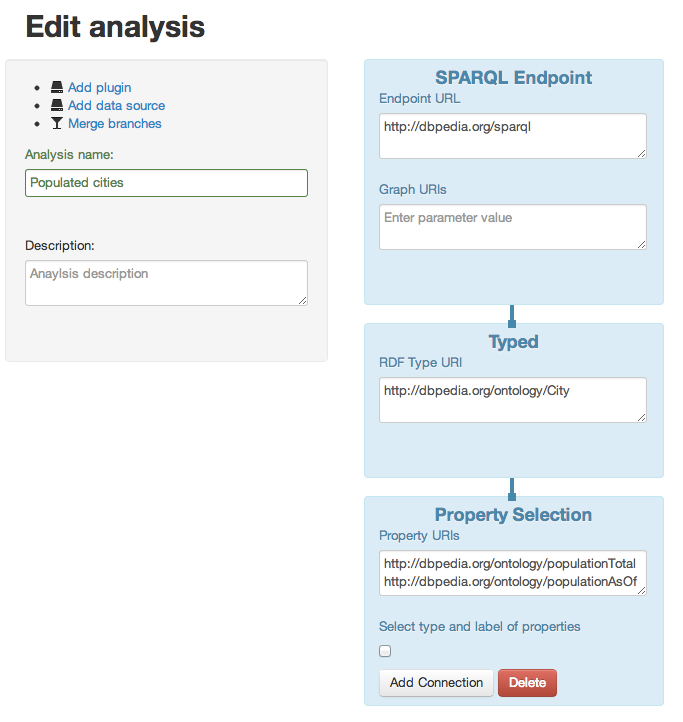
\includegraphics[width=100mm]{img/payola-exp-01-step1.png}
  \caption{An analytical pipeline made to~extract population data from the~DBPedia.}
  \label{fig:dbpedia-pop-anal}
\end{figure}

With the~preview size set to~20, the~preview is~shown as~pictured in~Figure~\ref{fig:payola-exp-01-preview}. In~this case, the~transformation pattern 
is very simple, as~shown in~Figure~\ref{fig:payola-exp-01-selection}. As~a 
result, the~system will apply the~following query to~transform the~data into~the
Data Cube Vocabulary standard:

\begin{figure}
  \centering
  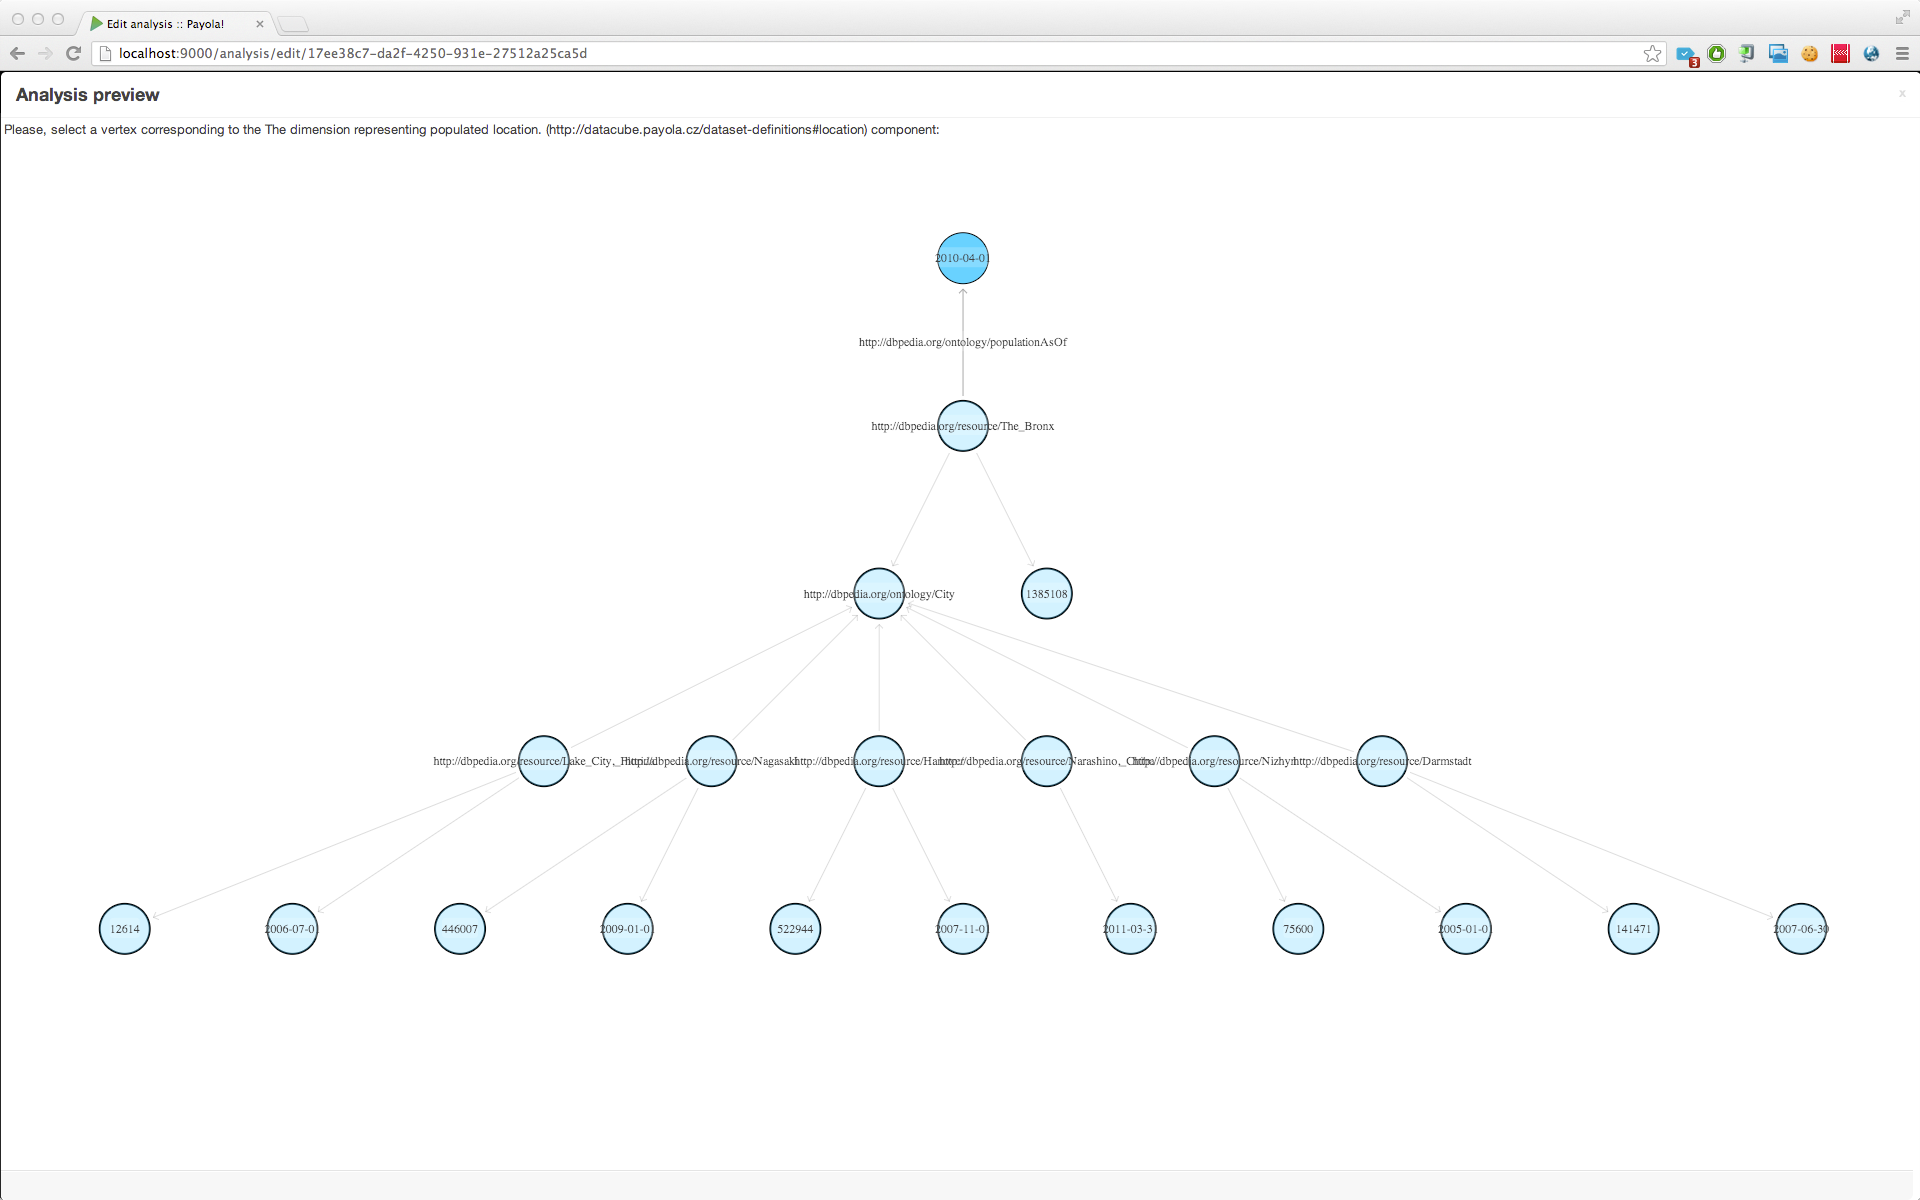
\includegraphics[width=140mm]{img/payola-exp-01-preview.png}
  \caption{An analytical pipeline preview used for a~pattern selection.}
  \label{fig:payola-exp-01-preview}
\end{figure}

\begin{figure}
  \centering
  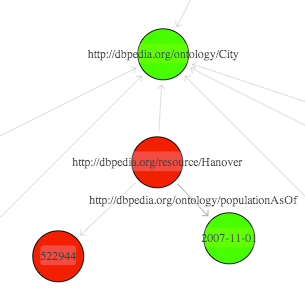
\includegraphics[width=50mm]{img/payola-exp-01-selection.png}
  \caption{An example provided by~the user in~a form of~a pattern.}
  \label{fig:payola-exp-01-selection}
\end{figure}

\scriptsize
\begin{verbatim}
  CONSTRUCT {
     []  a~ <http://purl.org/linked-data/cube#Observation> ;
         <http://purl.org/linked-data/cube#dataSet> <http://live.payola.cz/analysis/...> ;
         <http://datacube.payola.cz/dataset-definitions#location> ?v1 ;
         <http://datacube.payola.cz/dataset-definitions#period> ?v3 ;
         <http://datacube.payola.cz/dataset-definitions#populationSize> ?v4 .
     } where {
         {
             SELECT DISTINCT ?v1 ?v3 ?v4 {
                ?v1 <http://www.w3.org/1999/02/22-rdf-syntax-ns#type> ?v2 .
                ?v1 <http://dbpedia.org/ontology/populationAsOf> ?v3 .
                ?v1 <http://dbpedia.org/ontology/populationTotal> ?v4 .
            }
       }
  } 
\end{verbatim}
\normalsize

The transformation is~made in~another step of~the analytical pipeline. The~whole evaluation is~done in~seconds. An~exact measurement would not be~conclusive since it~depends on~the actual load of~the DBPedia. The~endpoint 
returns in~about 150 entities no~matter what we~do because that is~the final
count of~entities with the~required properties.

As a~result, we~get a~dataset compliant with the~Data Cube Vocabulary standard. 
We made a~visualization of~the dataset in~both new visualizers. The~results are 
shown in~Figure~\ref{fig:payola-exp-01-vis} and Figure~\ref{fig:payola-exp-01-vis2}.

\begin{figure}
  \centering
  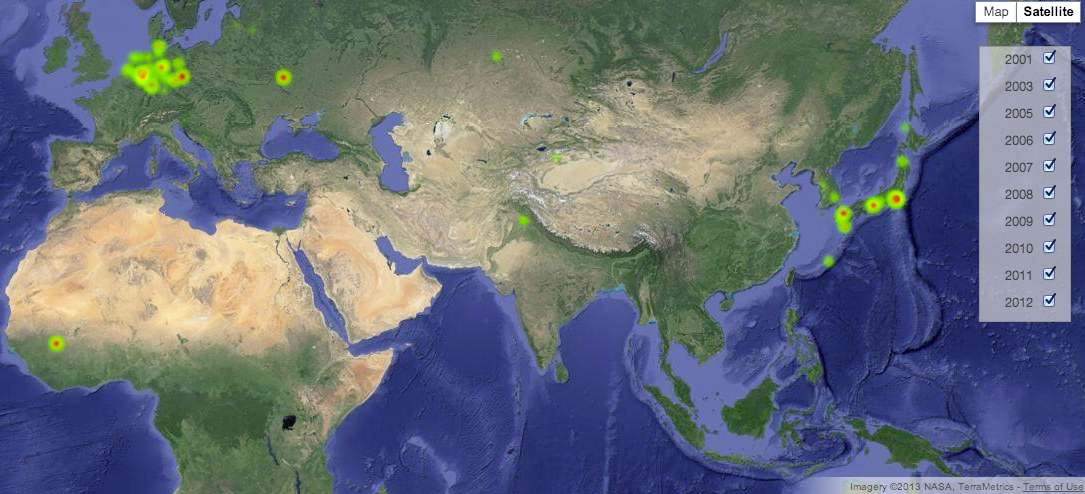
\includegraphics[width=140mm]{img/payola-exp-01-vis.png}
  \caption{Experiment 1: visualization with the~TimeHeatmap plugin.}
  \label{fig:payola-exp-01-vis}
\end{figure}

\begin{figure}
  \centering
  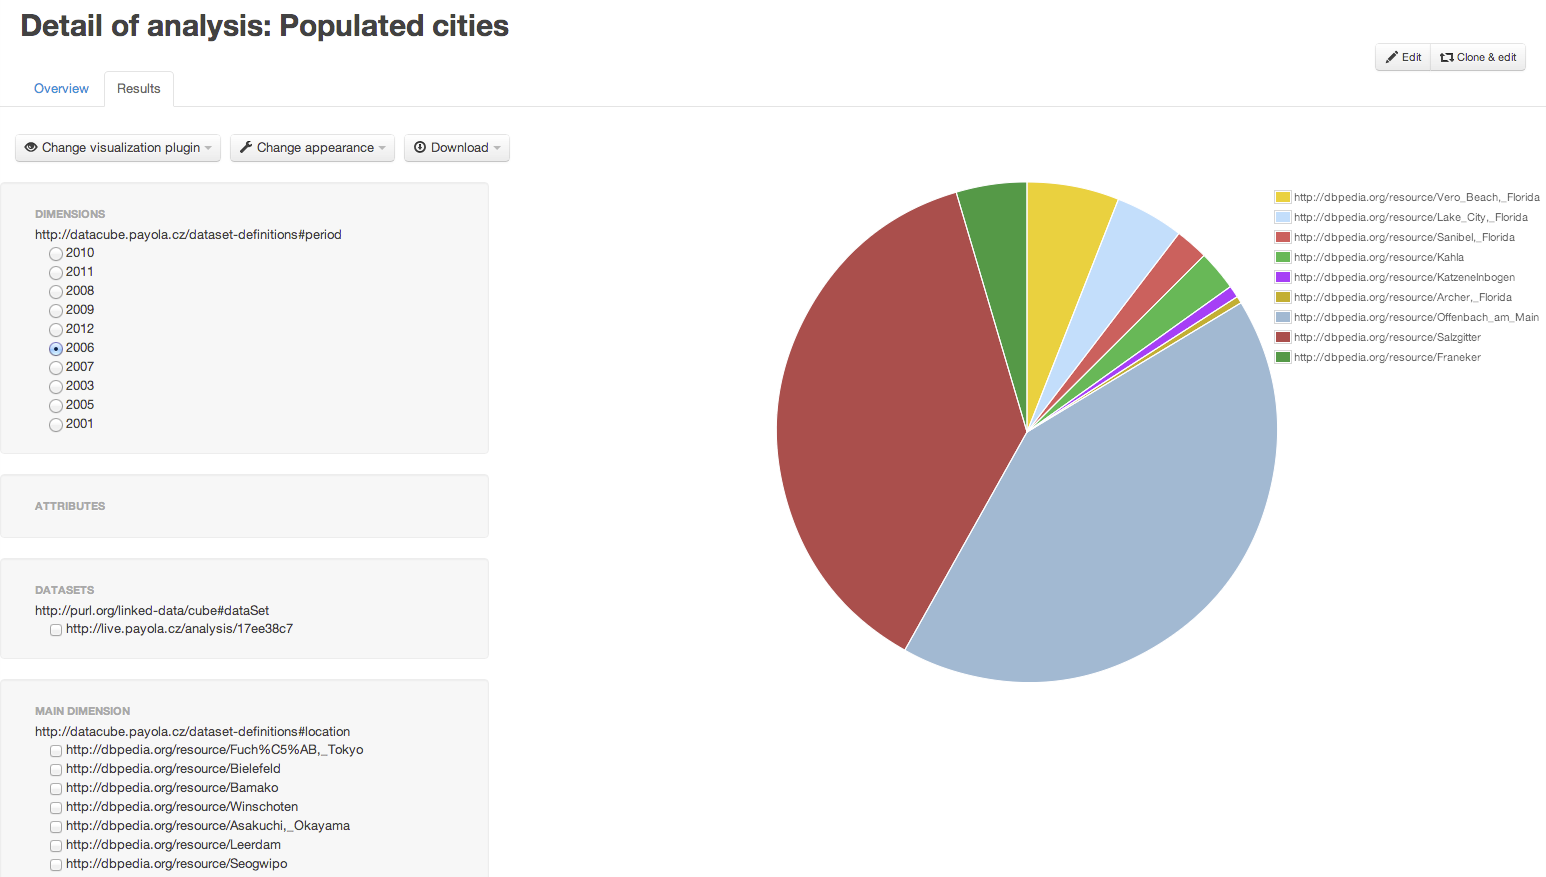
\includegraphics[width=140mm]{img/payola-exp-01-vis2.png}
  \caption{Experiment 1: visualization with the~Universal DataCube plugin.}
  \label{fig:payola-exp-01-vis2}
\end{figure}

In this experiment, we~proved that the~system is~capable of~converting an~arbitrary RDF dataset to~a format compliant with the~Data Cube Vocalbulary 
standard. We~took advantage of~the integration with the~Payola application in~order to~obtain a~meaningful preview.

The system performed well on~the dataset provided by~the DBPedia endpoint, but 
it is~important to~remember that the~endpoint returned a~small amount of~resources. The~quality of~the DBPedia datasets differs a~lot and many 
statistical data are present in~a non--user--friendly form, e.g. while using the~property~\texttt{2000pop}. It~might be~interesting to~use Payola to~discover 
all those properties and build an~analytical pipeline, which will unify all the~approaches. When unified, the~implemented system can be~used in~order to~transform the~data into~the~form of~DCV and/or visualize those.

We have also shown that our visualizers work with real--life data. Based on~what we~have experienced, we~will propose some future user experience 
improvements in~Chapter~\ref{ch:future}. One of~those is~optimizing a~longer running 
geocoding process, which transforms the~city names into~GPS cooridinates.

\section{COINS -- UK~government spending}
Many organizations including governments produce a~lot of~statistical datasets 
focused on~spendings. Therefore, we~wanted to~examine the~behaviour of~the 
system when applied on~such a~dataset. We~chose to~use a~dataset named 
COINS~\cite{coins}. It~is the~database for UK~Government expenditure.

The \url{data.gov.uk} project also made the~dataset available in~a form of~Linked 
Data. Moreover, it~is published in~a form compliant with Data Cube Vocabulary.
Therefore, it~is not necessary to~do a~transformation of~the dataset. But we~tried to~use the~implemented system to~extract the~data from the~original 
dataset.

It is~possible to~use only the~universal visualizer to~visualize the~data 
contained in~the dataset, but we~would need to~extract them manually. In~fact, 
we tried to~do that and we~had to~construct a~SPARQL query, which is~shown in
Figure~\ref{fig:custom-coins-query}. It~allows us~to extract the~data for a~specific data structure 
definition and visualize them. The~result of~such a~visualization is~shown in~Figure~\ref{fig:payola-exp-02}. 

\begin{figure}
  \centering
  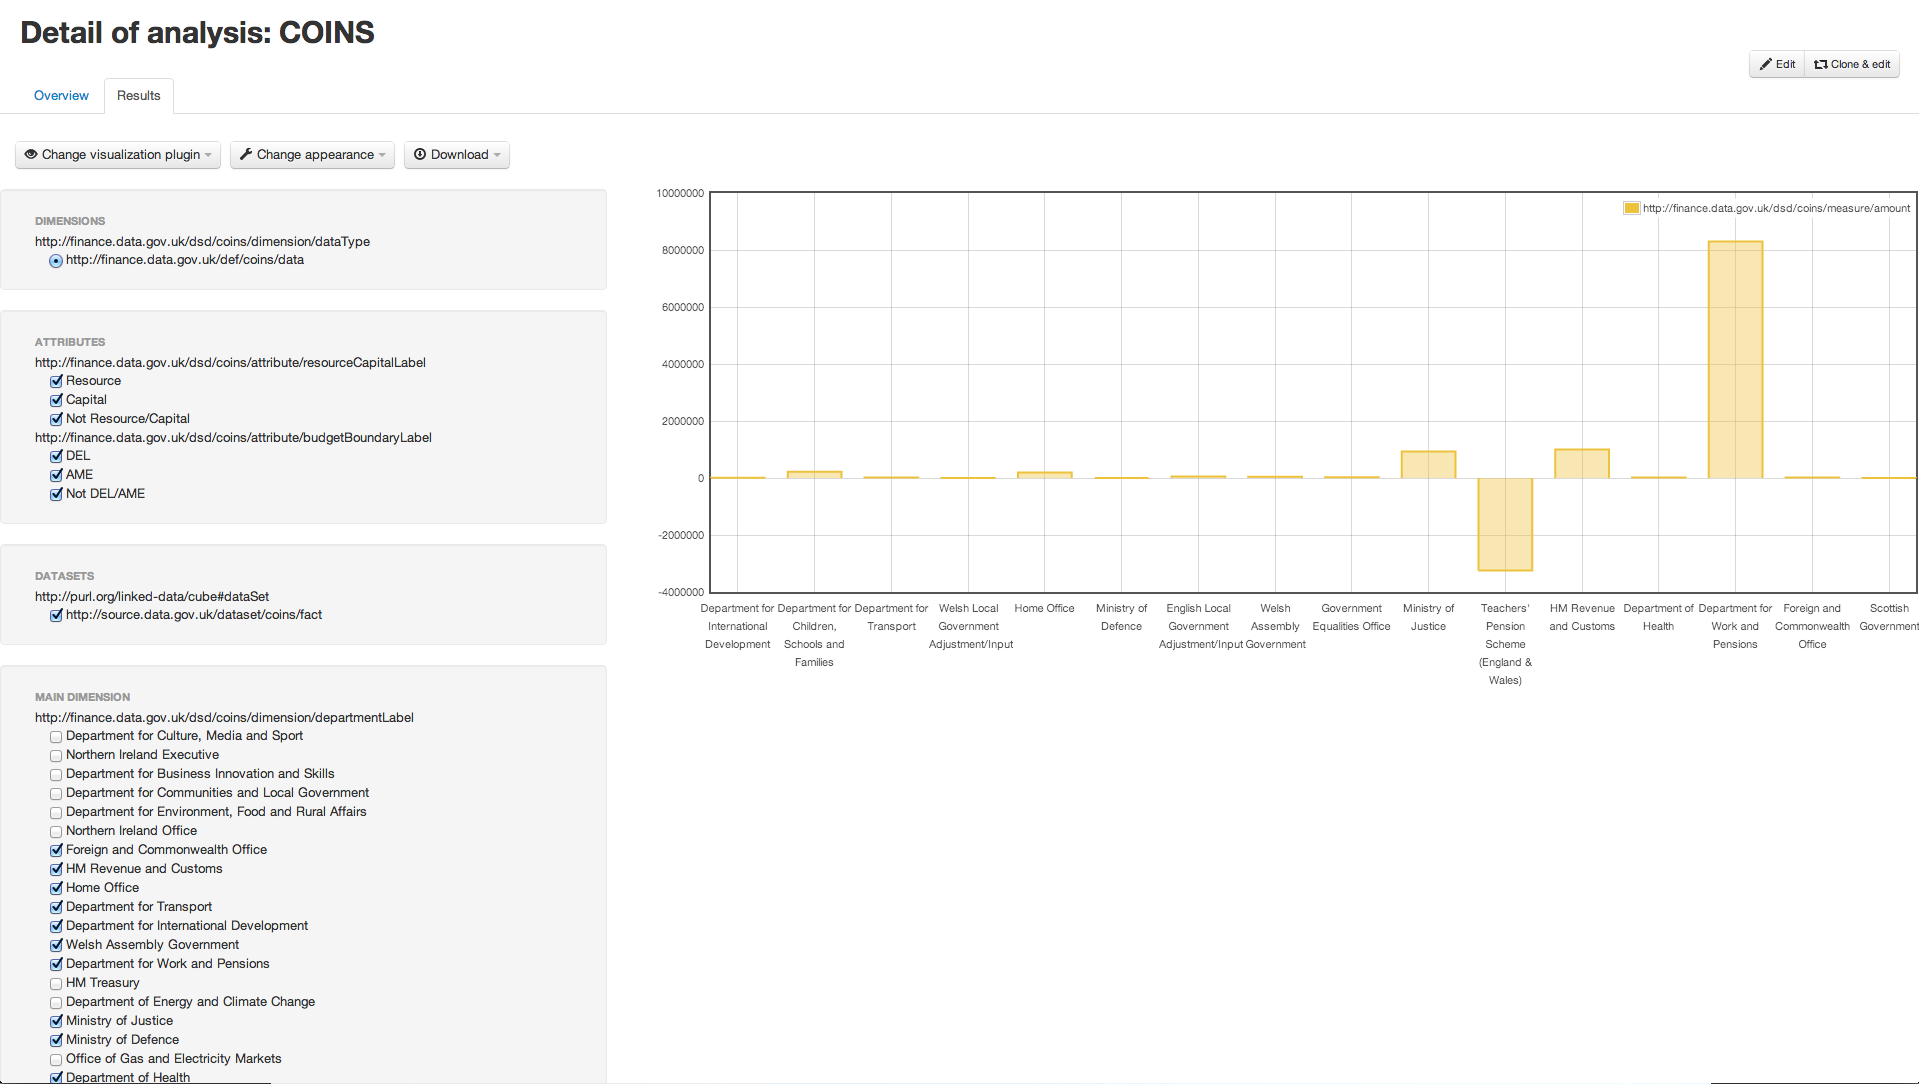
\includegraphics[width=140mm]{img/payola-exp-02.png}
  \caption{Experiment 2: visualization of~a custom query with the~Universal DataCube plugin.}
  \label{fig:payola-exp-02}
\end{figure}

\begin{figure}
  \centering
  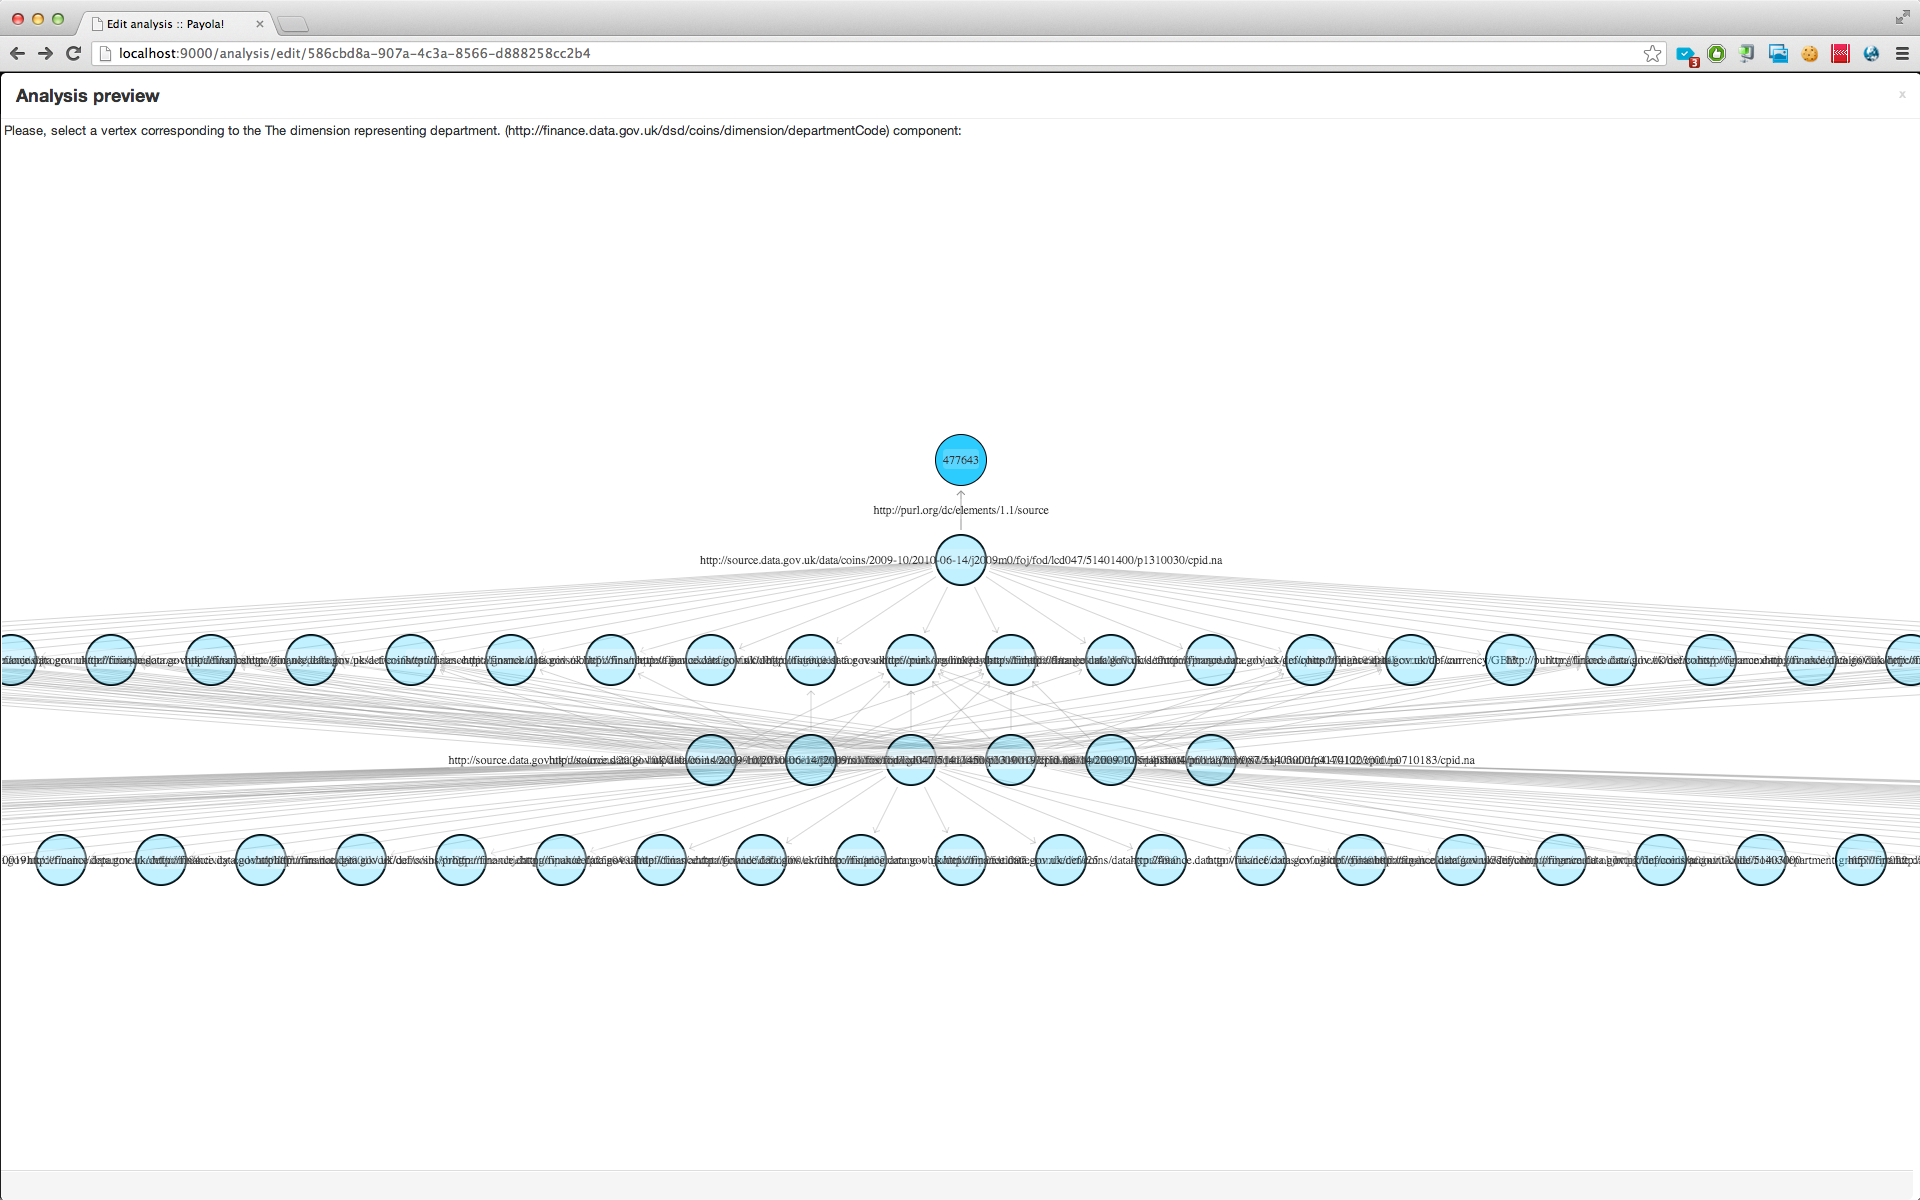
\includegraphics[width=140mm]{img/payola-exp-02-pattern.png}
  \caption{Experiment 2: Selecting an~exemplary pattern in~a complex graph might be~difficult, yet possible.}
  \label{fig:payola-exp-02-pattern}
\end{figure}

\begin{figure}
  \centering
  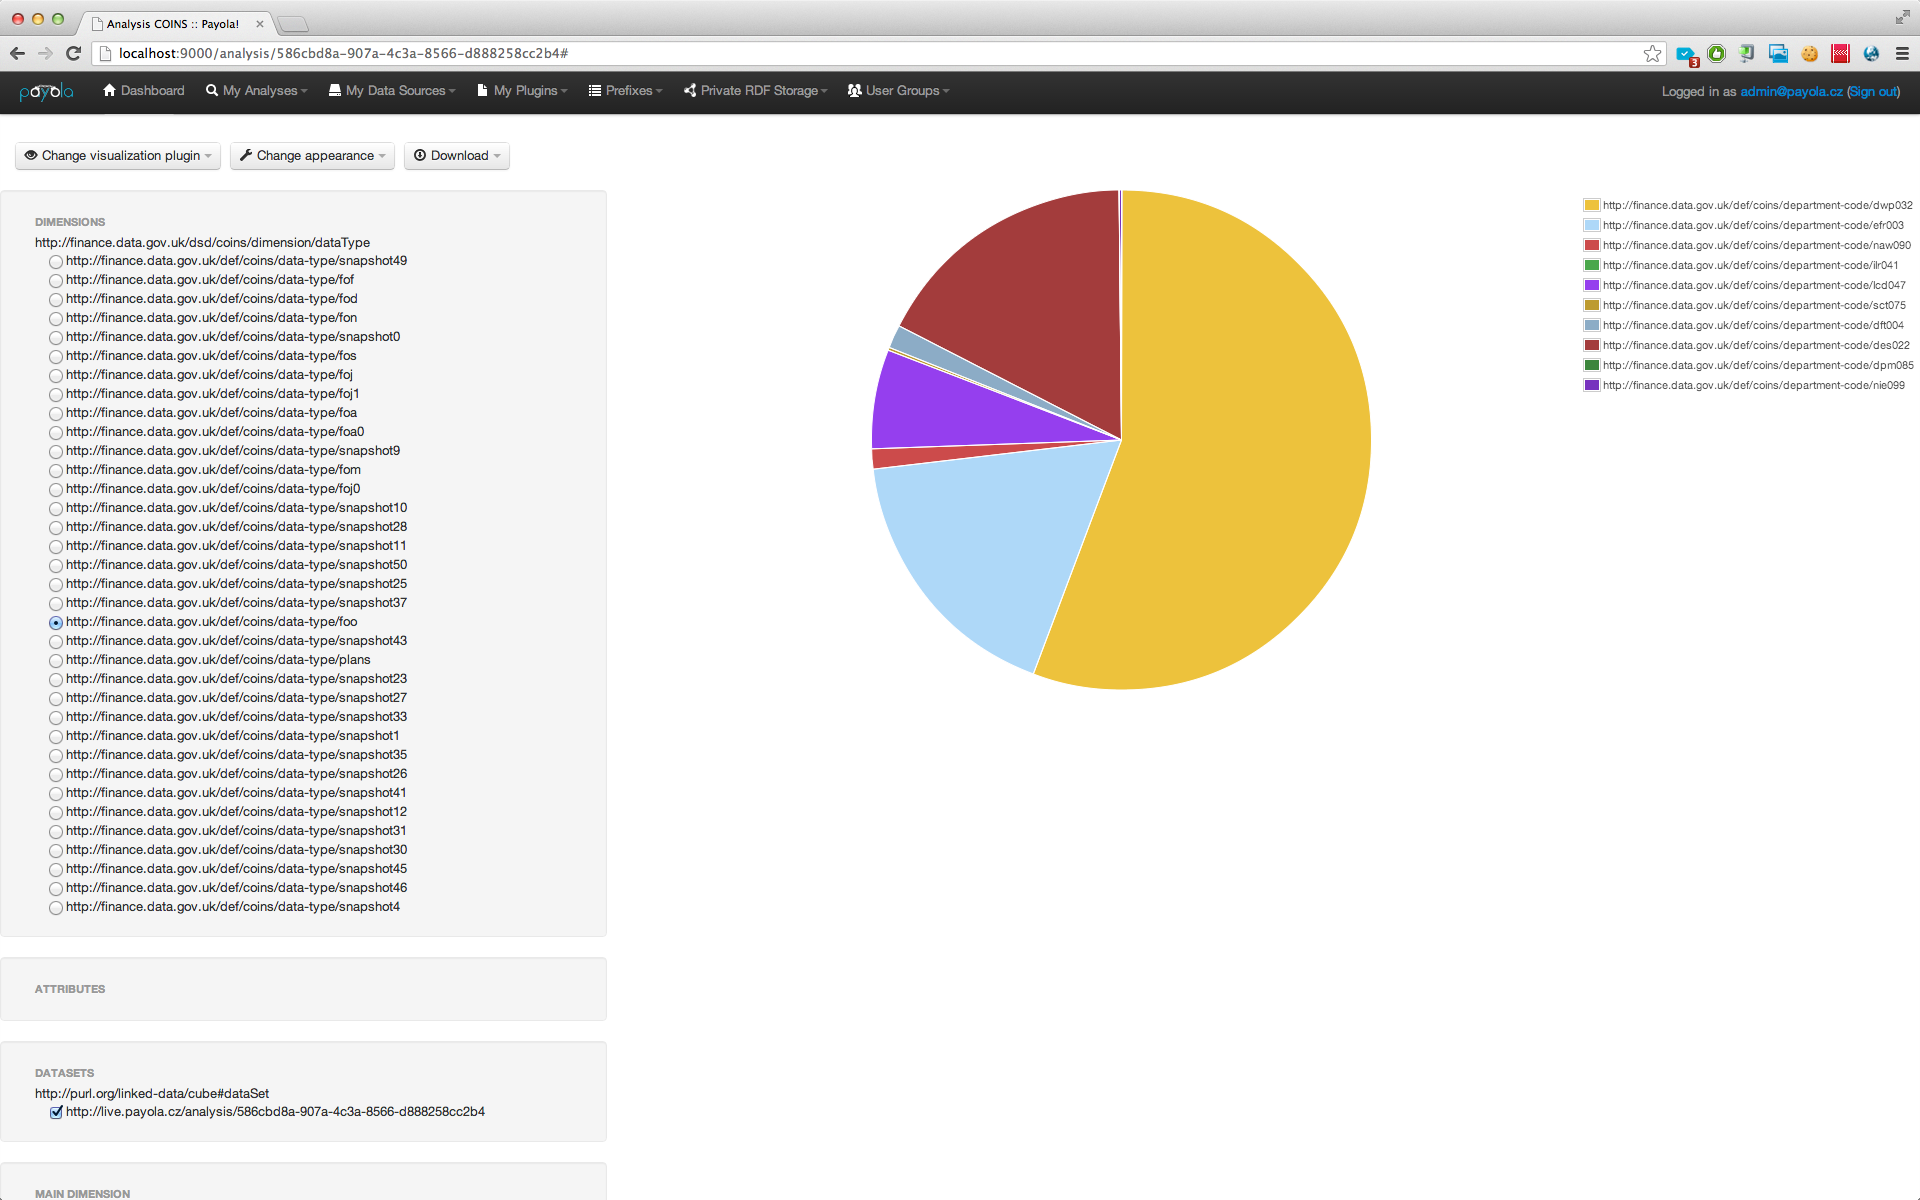
\includegraphics[width=140mm]{img/payola-exp-02-result.png}
  \caption{Experiment 2: Visualization of~the extracted dataset.}
  \label{fig:payola-exp-02-result}
\end{figure}

\begin{figure}
  \scriptsize
\begin{verbatim}
PREFIX  coins-dimension: <http://finance.data.gov.uk/dsd/coins/dimension/>
PREFIX  coins-measure: <http://finance.data.gov.uk/dsd/coins/measure/>
PREFIX  source: <http://source.data.gov.uk/>
PREFIX  coins-attribute: <http://finance.data.gov.uk/dsd/coins/attribute/>
PREFIX  qb:   <http://purl.org/linked-data/cube#>

CONSTRUCT 
  { ?obs qb:dataSet ?ds .
    ?obs a~qb:Observation .
    ?obs coins-dimension:dataType <http://finance.data.gov.uk/def/coins/data-type/outturn> .
    ?obs coins-measure:amount ?amount .
    ?obs coins-dimension:departmentLabel ?deptLongName .
    ?obs coins-attribute:budgetBoundaryLabel ?boundaryLabel .
    ?obs coins-attribute:resourceCapitalLabel ?rcLabel . }

WHERE
  { ?obs qb:dataSet ?ds .
    ?obs coins-dimension:departmentCode ?dept .
    ?obs coins-dimension:dataType <http://finance.data.gov.uk/def/coins/data-type/outturn> .
    ?obs coins-measure:amount ?amount .
    ?obs coins-attribute:budgetBoundary ?boundary .
    ?obs coins-attribute:resourceCapital ?rc
    GRAPH <http://source.data.gov.uk/finance/coins/2010-06-14/schema>
      { ?boundary <http://www.w3.org/2000/01/rdf-schema#label> ?boundaryLabel .
        ?rc <http://www.w3.org/2000/01/rdf-schema#label> ?rcLabel .
        ?dept <http://www.w3.org/2000/01/rdf-schema#comment> ?deptLongName
      }
  }
\end{verbatim}
\caption{A custom SPARQL query used to~extract DCV from the~COINS dataset.}
\label{fig:custom-coins-query}
\end{figure}

As stated before, we~tried to~use the~implemented system in~order to~obtain 
similar results. Since the~original dataset is~very large, we~had to~prepare an~analysis in~order to~get a~reasonable preview for a~pattern selection. The~analysis contained only one step. We~added a~SPARQL query plugin. The~query is~presented
in Figure~\ref{fig:coins-query-narrow}.

\begin{figure}
  \scriptsize
\begin{verbatim}
  CONSTRUCT { ?o ?p ?x }
  WHERE
  { ?o qb:dataSet <http://source.data.gov.uk/dataset/coins/fact-table-extract-2009-10> ;
        ?p ?x .
  }
\end{verbatim}
\caption{A custom SPARQL query used for narrowing the~original dataset.}
\label{fig:coins-query-narrow}
\end{figure}

By executing such a~query, we~obtained all triples from the~endpoint 
related to~the specified dataset. We~made a~strong constraint for bringing 
down the~volume of~returned entries. By~using the~\texttt{qb:dataSet} property, 
we automatically filtered the~observations.

Despite the~narrowed dataset, the~preview was still too large 
for the~resulting visualization to~be well--arranged. A~screenshot of~the 
preview can be~seen in~Figure~\ref{fig:payola-exp-02-pattern}. After a~while,
we managed to~select the~desired 
pattern. The~SPARQL query shown in~Figure~\ref{fig:coins-pattern-result} was 
constructed.

\begin{figure}
  \scriptsize
\begin{verbatim}
  CONSTRUCT {
    [] a~<http://purl.org/linked-data/cube#Observation> ;
    <http://purl.org/linked-data/cube#dataSet> <http://live.payola.cz/analysis/...> ;
    <http://finance.data.gov.uk/dsd/coins/dimension/departmentCode> ?v2 ;
    <http://finance.data.gov.uk/dsd/coins/dimension/dataType> ?v3 ;
    <http://finance.data.gov.uk/dsd/coins/measure/amount> ?v4 .
} WHERE {
    {
        SELECT DISTINCT ?v2 ?v3 ?v4 {
            ?v1 <http://finance.data.gov.uk/dsd/coins/dimension/departmentCode> ?v2 .
            ?v1 <http://finance.data.gov.uk/dsd/coins/dimension/dataType> ?v3 .
            ?v1 <http://finance.data.gov.uk/dsd/coins/measure/amount> ?v4 .
        }
    }
} 
\end{verbatim}
\caption{A SPARQL query constructed based on~the pattern selection dialog.}
\label{fig:coins-pattern-result}
\end{figure}

As one can see, the~query differs from the~one we~were about to~simulate. We~did not select available labels. On~the other hand, we~obtained a~more general 
query, which does not fix a~value of~the \texttt{dataType} dimension. That means 
that the~user is~able to~slice the~results of~such an~analysis with the~universal 
visualizer in~order to~obtain the~same visualization as~was in~the case of~the custom 
query. Moreover, they are able to~explore a~much wider range of~data.  

\begin{sloppypar}
Unfortunately, as~the original dataset is~way too large it~was not possible to~fetch all the~related data. The~SPARQL endpoint \mbox{\url{http://openuplabs.tso.co.uk/}}
is placed behind an~Apache proxy, which monitors the~load of~the underlying 
triplestore caused by~executing a~query. After a~while we~hit the~limit and had a~restricted access to~the endpoint for a~few minutes. Therefore, we~had to~limit 
the size of~the extracted dataset. We~managed to~get $10000$ in~the Payola's 
default limit (30 seconds). Most of~the time was spent on~obtaining all the~data from the~endpoint, the~extraction to~DCV was completed in~a matter of~seconds. Also, the~universal visualizer performed well on~a dataset that large.
We made a~screenshot of~a visualization that was prepared during this experiment.
It can be~seen in~Figure~\ref{fig:payola-exp-02-result}.
\end{sloppypar}

We learnt that the~system is~capable of~mapping larger datasets in~a reasonable 
time. But we~also found out that the~preview mechanism will need further 
modifications in~order to~handle larger previews in~a more user--friendly way. 
Performance of~the universal visualizer was acceptable for the~user interface 
responded continuously without any lags. However, we~hit the~limit of~the 
endpoint and were not able to~obtain the~complete dataset. 

The proper way of~working with this dataset would require a~fully faceted 
browser connected directly to~the original SPARQL endpoint. Since it~contains 
DCV data, the~system would be~able to~automatically discover used vocabularies 
and offer them to~the user. On~the other hand, the~vocabularies are not published
separately, which made our task a~bit harder. Implementing an~advanced browser
with an~exploration mode will definitely become the~next step in~the future work. It~would be~very useful to~give the~user a~tool, which will help them 
discover vocabularies and related data in~datasets, which are already compliant 
with Data Cube Vocabulary.

The recommended way of~solving the~large dataset problem with the~current state of~the system
is to~place the~DCV 
plugin into~a~more suitable point. The~preceding operations should narrow the~dataset more naturally by~setting semantical constraints.

In this experiment, we~tried to~use the~implemented system in~a slightly 
different use case. We~used it~in order to~extract a~dataset which is~already in~a form of~Data Cube Vocabulary. Despite the~fact that the~tool was not 
originally meant for this, we~managed to~fulfill our goal. On~the other hand, 
we discovered some user experience flaws, which will be~eliminated in~the future 
development of~the whole Payola framework.

\section{Czech public contracts}
As we~are able to~access the~data related to~public contracts realized in~the 
Czech Republic, we~want to~demonstrate on~them the~possibilities of~the implemented system.
The dataset was created by~scraping website produced by~an online system focused 
on publishing details about public contracts. Therefore, the~form of~the data is~natural and does not come out from a~statistical form.

At first, we~wanted to~extract the~data by~using a~very simple analysis
containing a~sole plugin, an~\emph{ontological filter}. Unfortunately, the~length
of the~generated SPARQL query exceeds the~limit of~the queried SPARQL endpoint.
We extracted the~generated query and tried to~shorten it~by applying prefixes 
and removing whitespace characters. However, after overcoming this challenge, we~hit another limit --- the~underlying Virtuoso endpoint refused to~run the~query 
due to~a large estimated time of~transaction execution.

That is~why we~had to~construct a~custom query in~order to~obtain the~required 
data for making a~preview and a~transformation. We~designed the~query to~gather as~much data as~possible while keeping the~important statistical facts in~all of~the returned entries. The~query is~shown in~Figure~\ref{fig:contracts-query}. It~returns the~details of~about $40000$ public 
contracts.

\begin{figure}
  \scriptsize
  \begin{verbatim}
PREFIX contract: <http://purl.org/procurement/public-contracts#>
PREFIX rdfs: <http://www.w3.org/2000/01/rdf-schema#>
PREFIX dcterms: <http://purl.org/dc/terms/>
prefix vcard: <http://www.w3.org/2006/vcard/ns#> 
prefix gr:	<http://purl.org/goodrelations/v1#> 
prefix ns4:	<http://purl.org/procurement/public-contracts-eu#>

CONSTRUCT 
{
   ?v1 a~contract:Contract .
   ?v1 contract:location ?vloc .
   ?vloc rdfs:label ?locLabel .
   ?vloc ns4:hasParentRegion ?reg .
   ?v1 contract:startDate ?v17 .
   ?v1 contract:estimatedPrice ?ep .
   ?ep gr:hasCurrencyValue	?epv.
}
WHERE
{
   ?v1 a~contract:Contract .
   ?v1 contract:location ?vloc .
   ?vloc rdfs:label ?locLabel .
   ?vloc ns4:hasParentRegion ?reg .
   ?v1 contract:startDate ?v17 .
   ?v1 contract:estimatedPrice ?ep .
   ?ep gr:hasCurrencyValue	?epv.
}
  \end{verbatim}
  \caption{A query constructed to~obtain a~dataset containing desired data.}
  \label{fig:contracts-query}
\end{figure}

We also had to~construct a~custom Data Cube vocabulary with a~data structure 
definition. We~present the~vocabulary in~Figure~\ref{fig:contracts-dcv}.

\begin{figure}
  \scriptsize
  \begin{verbatim}
@prefix rdf:     <http://www.w3.org/1999/02/22-rdf-syntax-ns#> .
@prefix rdfs:    <http://www.w3.org/2000/01/rdf-schema#> .
@prefix xsd:     <http://www.w3.org/2001/XMLSchema#> .
@prefix payola-dcv:   <http://datacube.payola.cz/dataset-definitions#> .
@prefix qb:              <http://purl.org/linked-data/cube#> .
@prefix sdmx:            <http://purl.org/linked-data/sdmx#> .
@prefix sdmx-concept:    <http://purl.org/linked-data/sdmx/2009/concept#> .
@prefix sdmx-dimension:  <http://purl.org/linked-data/sdmx/2009/dimension#> .
@prefix sdmx-measure:    <http://purl.org/linked-data/sdmx/2009/measure#> .
@prefix pc: <http://purl.org/procurement/public-contracts#> .
@prefix ns4: <http://purl.org/procurement/public-contracts-eu#> .
@prefix nuts:     <http://ec.europa.eu/eurostat/ramon/ontologies/geographic.rdf#> .

payola-dcv:ContractsDatastructureDefinition a~qb:DataStructureDefinition ;
  rdfs:label "The definition of~the DS~of a~dataset containing information about public contracts."@en ;
  # Dimensions
  qb:component [
    qb:dimension payola-dcv:location;
    qb:order 1 ;
    rdfs:label "The dimension representing location, where the~money was spent."
  ] ;
  qb:component [  
    qb:dimension payola-dcv:period;
    qb:order 2 ;
    rdfs:label "The dimension representing the~time of~realizing the~contract."
  ] ;
  # Measure
  qb:component [
    qb:measure payola-dcv:price;
    rdfs:label "The measure representing the~price spent on~realizing the~contract."@en
  ] ;
  qb:component [
    qb:attribute payola-dcv:contract;
    rdfs:label "The attribute linking the~observation with a~corresponing contract."@en
  ] ;
  qb:component [
    qb:attribute payola-dcv:region;
    rdfs:label "The attribute specifying the~region, where the~contract was realized."@en
  ] ;
  qb:component [
    qb:attribute payola-dcv:currency;
    rdfs:label "Currency of~the price."@en
  ] .

payola-dcv:location a~rdf:Property, qb:DimensionProperty ;
  rdfs:label "reference location"@en ;
  qb:concept sdmx-concept:refArea .

payola-dcv:period a~rdf:Property, qb:DimensionProperty ;
  rdfs:label "reference period"@en ;
  qb:concept sdmx-concept:refPeriod .

payola-dcv:price a~rdf:Property, qb:MeasureProperty ;
  rdfs:label "price"@en ;
  rdfs:subPropertyOf sdmx-measure:obsValue ;
  rdfs:range xsd:nonNegativeInteger ;
  qb:concept sdmx-concept:valuation .

payola-dcv:contract a~rdf:Property, qb:AttributeProperty ;
  rdfs:label "corresponding public contract"@en ;
  rdfs:range pc:Contract ;
  qb:concept sdmx-concept:comment .
  
payola-dcv:region a~rdf:Property, qb:AttributeProperty ;
  rdfs:label "Parent NUTS region."@en ;
  rdfs:range nuts:NUTSRegion;
  qb:concept sdmx-concept:refArea .
  \end{verbatim}
  \caption{Public contracts data structure definition.}
  \label{fig:contracts-dcv}
\end{figure}

After we~had prepared all the~prerequisities, we~proceeded with transforming the~original dataset to~the form compliant with Data Cube Vocabulary. Based on~the 
data structure definition, we~created a~corresponding plugin, which was then 
inserted into~an~analysis. The~preview contained one of~the selected entries, 
therefore it~was an~easy task to~select a~mapping pattern. One step of~the 
pattern selection process is~pictured in~Figure~\ref{fig:contracts-pattern}.
As a~result, the~system gave us~the SPARQL query show in~Figure~\ref{fig:contracts-query-pattern}.

\begin{figure}
  \centering
  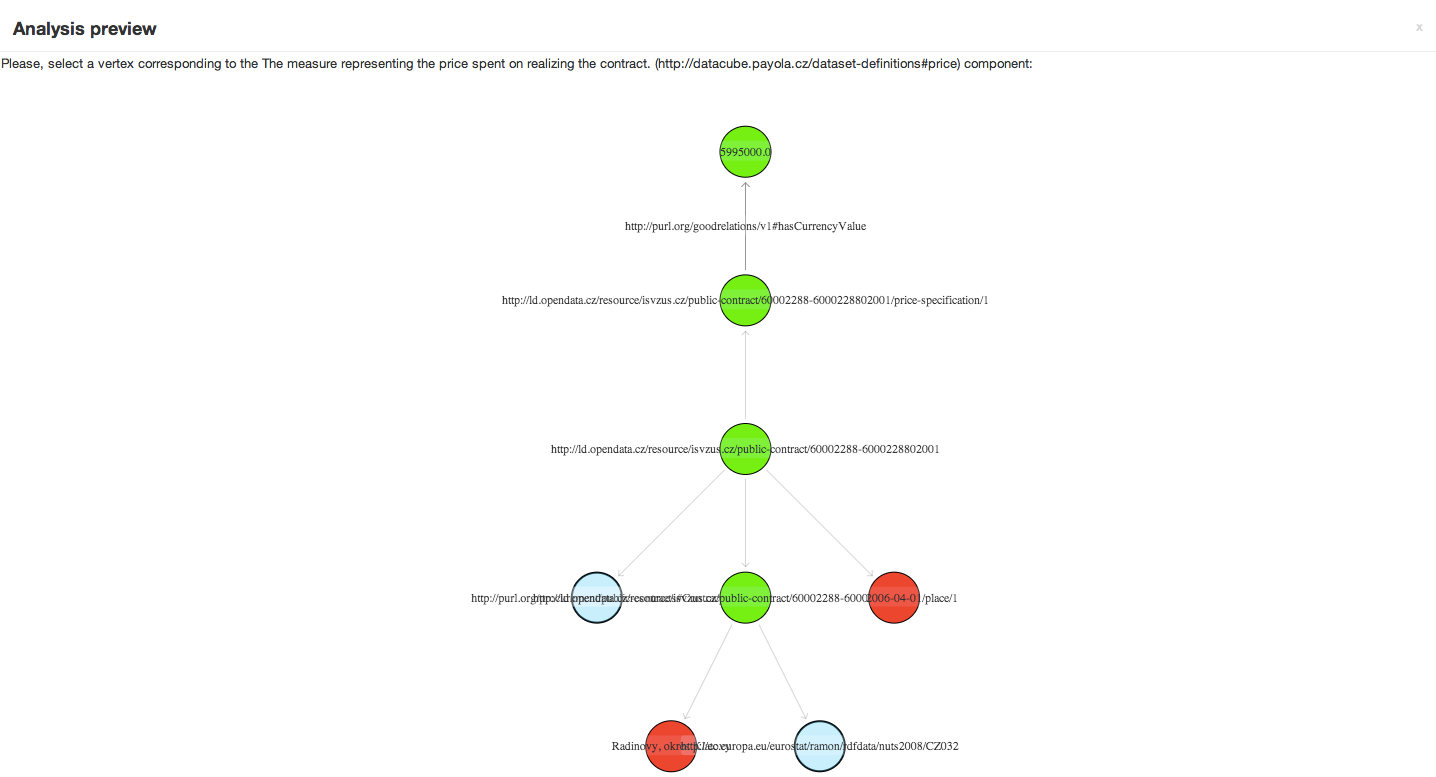
\includegraphics[width=140mm]{img/contracts-pattern.png}
  \caption{Experiment 3: Pattern selection.}
  \label{fig:contracts-pattern}
\end{figure}

\begin{figure}
  \scriptsize
  \begin{verbatim}
CONSTRUCT {
    [] a~<http://purl.org/linked-data/cube#Observation> ;
       qb:dataSet <http://live.payola.cz/analysis/...> ;
       <http://datacube.payola.cz/dataset-definitions#location> ?v2 ;
       <http://datacube.payola.cz/dataset-definitions#period> ?v4 ;
       <http://datacube.payola.cz/dataset-definitions#price> ?v6 ;
       <http://datacube.payola.cz/dataset-definitions#contract> ?v3 ;
       <http://datacube.payola.cz/dataset-definitions#region> ?v7 ;
} where {
   {
      SELECT DISTINCT ?v2 ?v4 ?v6 ?v3 ?v7 {
         ?v1 <http://www.w3.org/2000/01/rdf-schema#label> ?v2 .
         ?v3 <http://purl.org/procurement/public-contracts#location> ?v1 .
         ?v3 <http://purl.org/procurement/public-contracts#startDate> ?v4 .
         ?v3 <http://purl.org/procurement/public-contracts#estimatedPrice> ?v5 .
         ?v5 <http://purl.org/goodrelations/v1#hasCurrencyValue> ?v6 .
         ?v2 <http://purl.org/procurement/public-contracts-eu#hasParentRegion> ?v7 .
      }
   }
} 
  \end{verbatim}
  \caption{Experiment 3: Transformation query.}
  \label{fig:contracts-query-pattern}
\end{figure}

The conversion of~all the~resources in~the source lasted around 300 seconds. We~have noticed that it~took about 200 seconds to~make the~mapping itself, the~rest 
was spent on~fetching the~data.

We tried to~visualize the~dataset in~both implemented Data Cube visualizers. At~first, we~experimented 
with the~TimeHeatmap visualizer. While working with the~large dataset, we~experienced some user discomfort. The~UI was unresponsive for a~short period of~time
(that is~caused by~the single--threaded JavaScript processing concept and would require
involving Web Workers to~avoid). 
In order to~geocode the~locations from the~result, we~had to~increase the~maximum size of~a POST request allowed in~the application. We~present samples of~created visualizations in~Figure~\ref{fig:contracts-map-world} and 
Figure~\ref{fig:contracts-map-zoomed}.

The geocoding process was done in~an acceptable time, but the~size of~the 
dataset caused that the~Google Maps visualization had troubles with zooming. It~had to~recompute all the~40000 of~locations with every zoom.

\begin{figure}
  \centering
  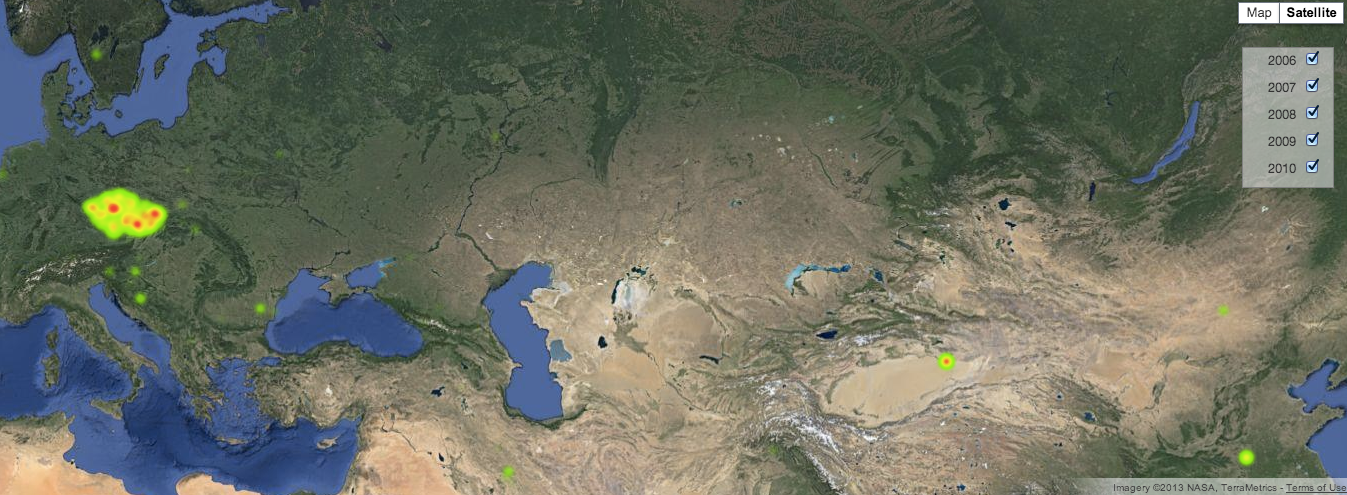
\includegraphics[width=140mm]{img/contracts-map-world.png}
  \caption{Experiment 3: Map expressing the~amount of~money spent by~the Czech Republic in~the world.}
  \label{fig:contracts-map-world}
\end{figure}

\begin{figure}
  \centering
  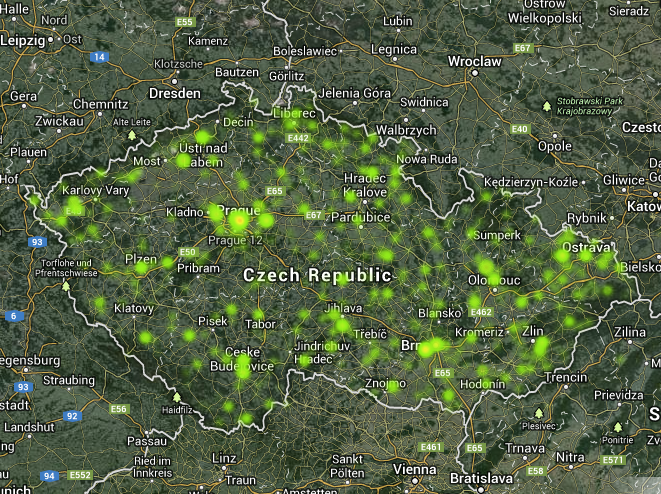
\includegraphics[width=100mm]{img/contracts-map-zoomed.png}
  \caption{Experiment 3: Map from Figure~\ref{fig:contracts-map-world} zoomed to~the level of~the Czech Republic.}
  \label{fig:contracts-map-zoomed}
\end{figure}

The size of~the dataset caused a~performance drop also in~the case of~the
Universal Data Cube visualizer. Despite the~fact, we~are able to~slice it~and 
take advantage of~the Data Cube Vocabulary format. An~example of~a visualization 
made by~the Universal Data Cube visualizer is~shown in~Figure~\ref{fig:contracts-uni-dcv}.

\begin{figure}
  \centering
  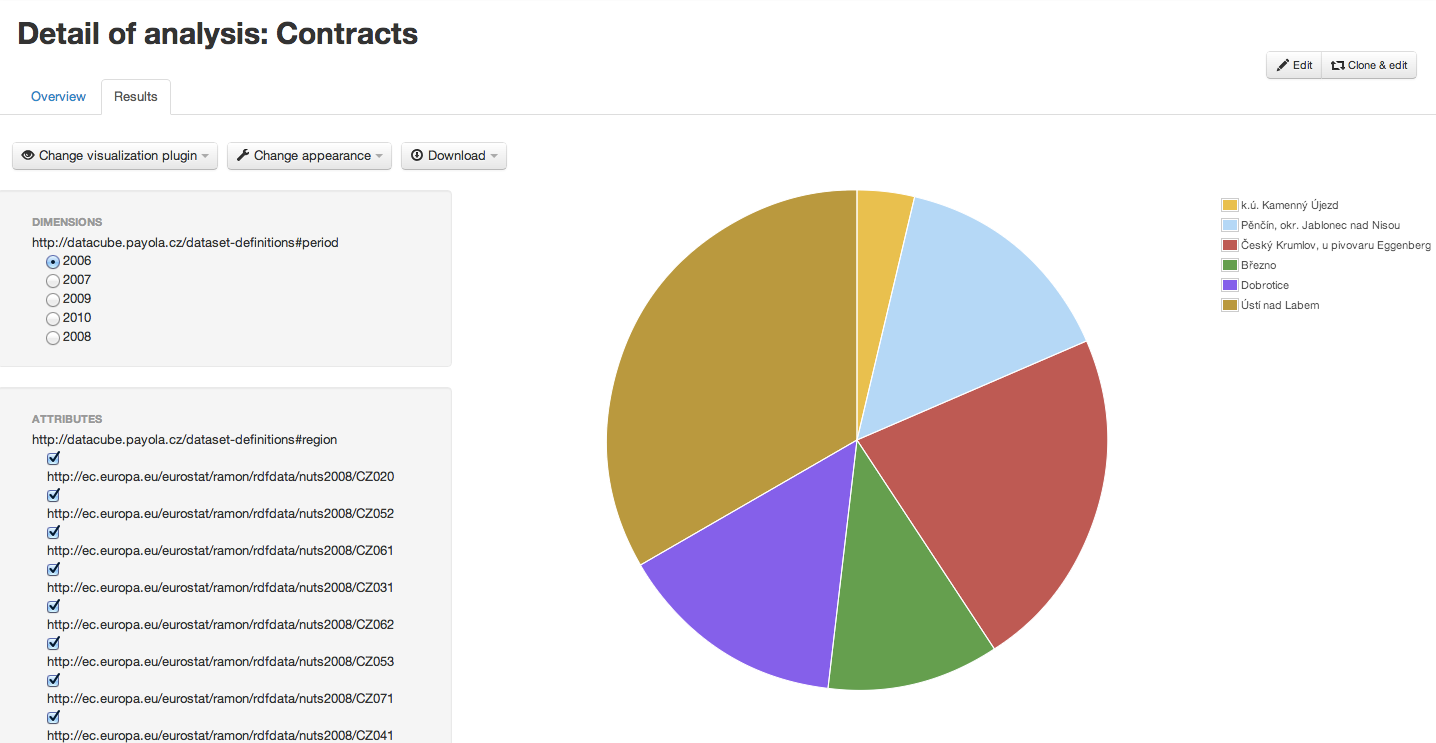
\includegraphics[width=140mm]{img/contracts-uni-dcv.png}
  \caption{Experiment 3: Universal Data Cube visualizer.}
  \label{fig:contracts-uni-dcv}
\end{figure}

In this experiment, we~confirmed that the~implemented system is~capable of~transforming an~arbitrary RDF dataset into~a~form compliant with a~selected Data 
Cube vocabulary. We~also examined the~system while working with a~larger 
dataset. We~confirmed some aforementioned assumptions about the~performance of~the system. Therefore, we~confirmed that we~have correctly identified all the~bottlenecks predicted while preparing the~proposal of~integrating the~system with Payola. 
We will account them in~the future improvements.

